\section{Web application}
\label{sec-webapplication}

\subsection{Server side/Back end}
\label{sec-webapplication-server}

The server is the core of the Geant4 validation system.
%It provides Web API for the clients to request data from PostgreSQL database and generates high quality plots on the fly when they are requested.
It is written in JavaScript using Node.js engine. Application data is stored in PostgreSQL DBMS provided by CERN Database On Demand (DBOD) service. Database schema is designed in a way to allow storing scatter plots and histograms with unlimited number of parameters. The server provides fast and efficient REST API for the clients.

To produce high quality plots we use own ROOT~\cite{ROOT} based C++ utility which uses data in our JSON format (see Appendix~\ref{adx:JSON-format}). It is not deeply integrated in the server infrastructure and can be used as a standalone console application. The utility supports scatter plots and 1D histograms with ability to plot on one canvas histograms with different binning and/or ratio plots. Plot axes scales are selected automatically, with ability to override them if necessary. User-defined styles for plots are also supported.
%It produces plots in all ROOT-supported formats with automatically adjusted (or manually set) axes scales, user styles (marker styles, colors, line width ...). 

%Node.js is an open-source, cross-platform JavaScript run-time environment that executes JavaScript code outside of a browser. Historically, JavaScript was used primarily for client-side scripting, in which scripts written in JavaScript are embedded in a webpage's HTML and run client-side by a JavaScript engine in the user's web browser. Node.js lets developers use JavaScript to write Command Line tools and for server-side scripting—running scripts server-side to produce dynamic web page content before the page is sent to the user's web browser. Consequently, Node.js represents a "JavaScript everywhere" paradigm, unifying web application development around a single programming language, rather than different languages for server side and client side scripts.

%Node.js has an event-driven architecture capable of asynchronous I/O. These design choices aim to optimize throughput and scalability in web applications with many input/output operations, as well as for real-time Web applications (e.g., real-time communication programs and browser games).

The schema of the client-server interactions is shown on the Fig.~\ref{fig:schema}. Both client and server side of the application use JSON for requests.

\begin{figure}[h]
    \centering
    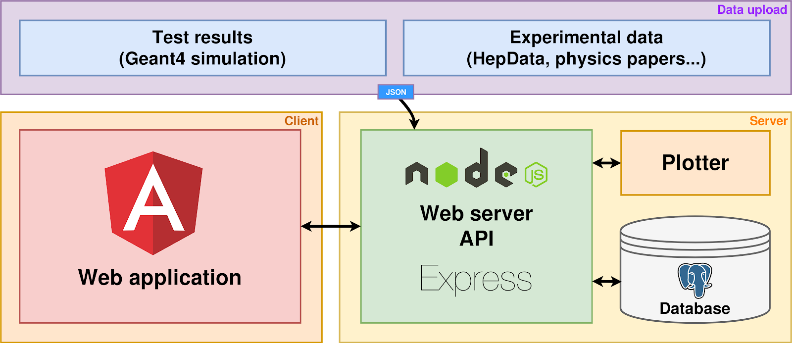
\includegraphics[width=0.8\textwidth,clip]{schema.png}
    \caption{Schema of the validation application}
    \label{fig:schema}
\end{figure}

\subsection{Client side/Front end}
\label{sec-webapplication-client}

Client side application is an AngularJS single page application (SPA). 

%AngularJS is a JavaScript-based open-source front-end web application framework mainly maintained by Google and by a community of individuals and corporations to address many of the challenges encountered in developing single-page applications. The JavaScript components complement Apache Cordova, a framework used for developing cross-platform mobile apps. It aims to simplify both the development and the testing of such applications by providing a framework for client-side model–view–controller (MVC) and model–view–viewmodel (MVVM) architectures, along with components commonly used in rich Internet applications.

Website contains 4 pages:

\begin{itemize}
    \item User layouts
    \item Statistical comparison
    \item Experimental data
    \item Page to search values in application's database
\end{itemize}

"User layouts" page (see Fig.~\ref{fig:layouts}) is designed for visual comparison of set of plots. It is possible to compare different versions between them and against experimental data. Also users can write their own templates and use them on the layouts page. Each plot on the page can be displayed in static and interactive mode. If two or more Geant4 versions are selected, one can also enable plotting the ratio.

\begin{figure}[h]
    \centering
    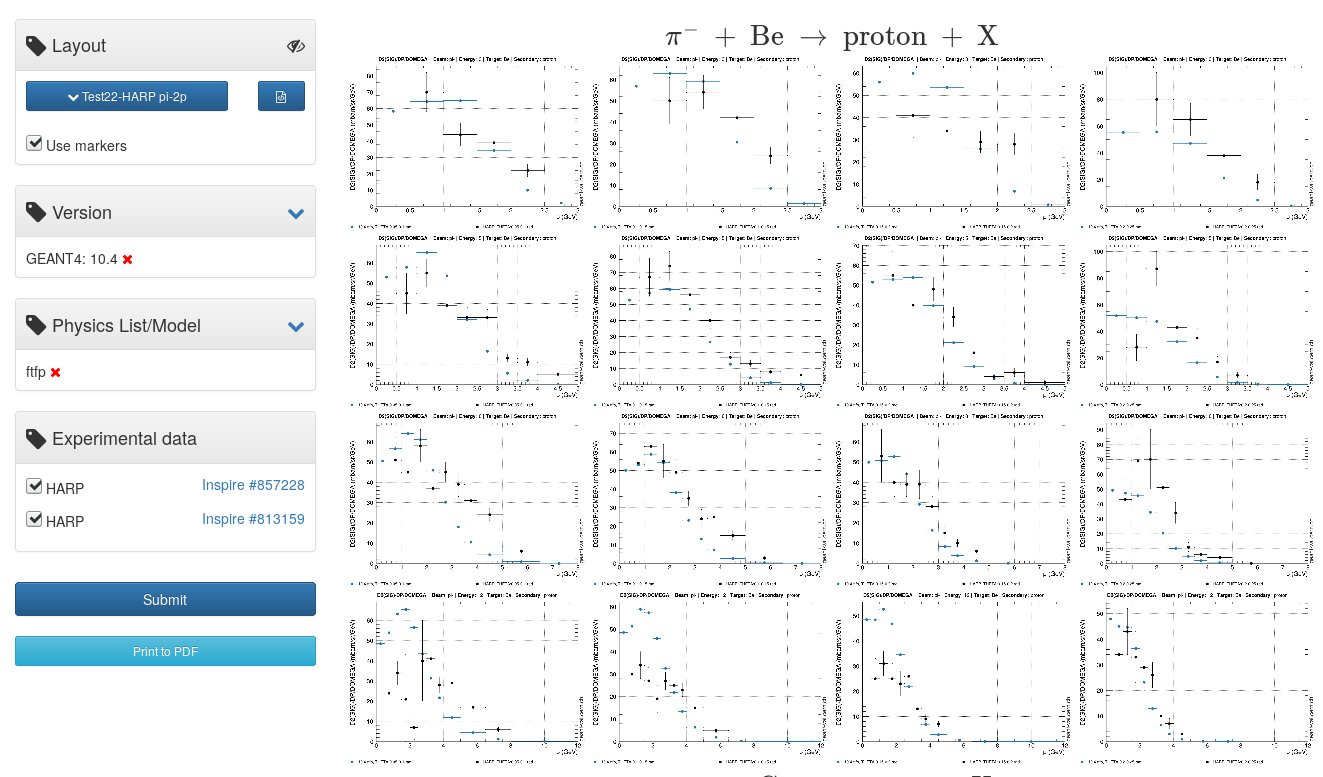
\includegraphics[width=0.8\textwidth,clip]{layouts.png}
    \caption{User layouts.}
    \label{fig:layouts}
\end{figure}

"Statistical comparison" page (see Fig.~\ref{fig:statcomparison}) allows performing statistical validation of Geant4 and experiments for given test. It displays pairs of plots for different versions with the same parameter values. For these pairs results of $\chi^2$ and Kolmogorov-Smirnov (KS) tests are displayed ($\chi^2/n.d.f.$, $\chi^2$ probability, KS and KS $\mathrm{Max(D)}$). All computations are performed on the client side in separate browser's processes using WebWorkers API. Implementation of $\chi^2$ and Kolmogorov-Smirnov tests is validated and gives the same results as ROOT framework.

\begin{figure}[h]
    \centering
    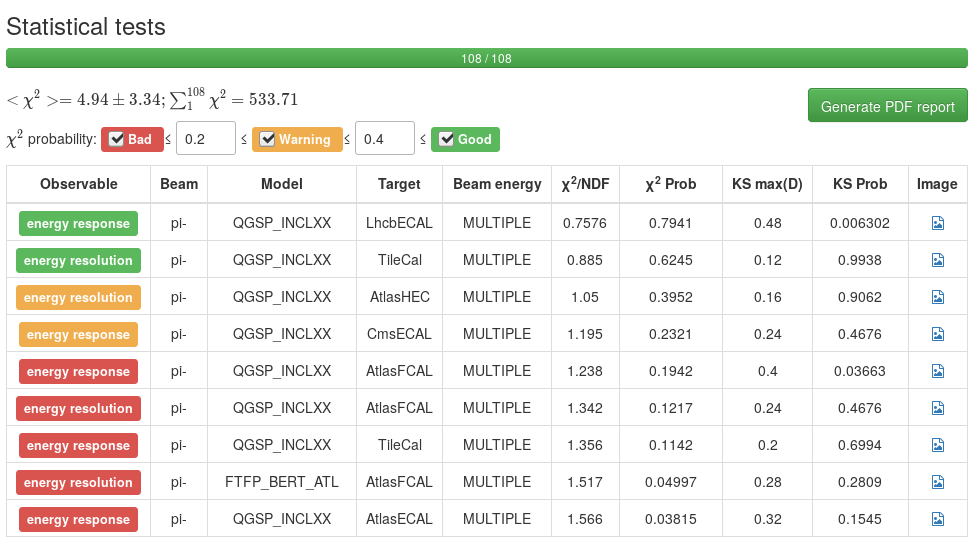
\includegraphics[width=0.8\textwidth,clip]{statcomparison.png}
    \caption{Statistical comparison.}
    \label{fig:statcomparison}
\end{figure}

On the "experiment data" page (see Fig.~\ref{fig:exppage}) one can see summary table of experimental data available in the application's database.
"Lookup table" page contains all predefined values, such as project names, versions, observables, particles, etc.

\begin{figure}[h]
    \centering
    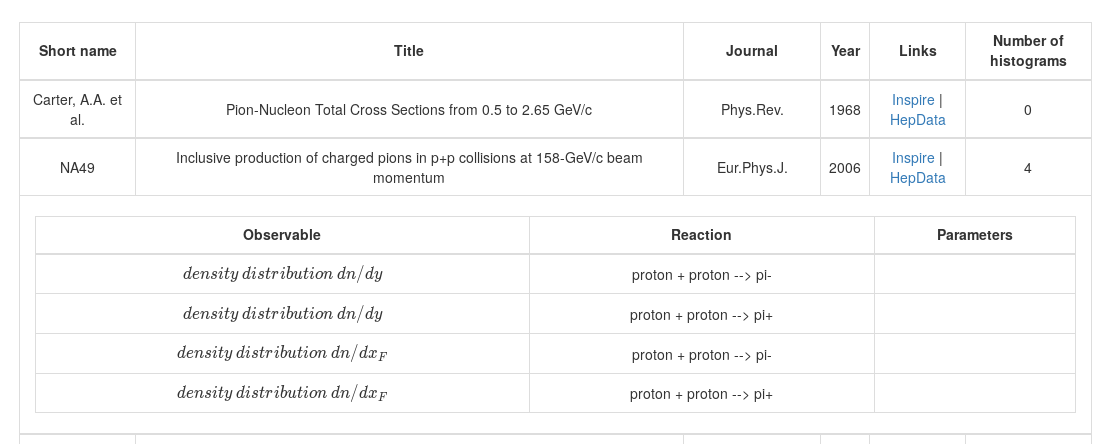
\includegraphics[width=0.8\textwidth,clip]{expdata.png}
    \caption{Available experimental data.}
    \label{fig:exppage}
\end{figure}

Each plot in the application can be viewed in interactive mode using JSROOT~\cite{JSROOT}, which allows changing axes ranges, scales and styles of the data "on the fly" in the same way as it can be done in ROOT. It is possible to export the plots in PNG, ROOT or EPS format to use them in articles or reports. For testing purposes it also provides JSON and Gnuplot output.

In order to restrict access to Geant4 testing releases, the application uses user authorization based on CERN Single-Sign-On service.

%Don't forget to give each section, subsection, subsubsection, and
%paragraph a unique label (see Sect.~\ref{sec-1}).

%For one-column wide figures use syntax of figure~\ref{fig-1}
%\begin{figure}[h]
% Use the relevant command for your figure-insertion program
% to insert the figure file.
%\centering
%\includegraphics[width=1cm,clip]{tiger}
%\caption{Please write your figure caption here}
%\label{fig-1}       % Give a unique label
%\end{figure}

%For two-column wide figures use syntax of figure~\ref{fig-2}
%\begin{figure*}
%\centering
% Use the relevant command for your figure-insertion program
% to insert the figure file. See example above.
% If not, use
%\vspace*{5cm}       % Give the correct figure height in cm
%\caption{Please write your figure caption here}
%\label{fig-2}       % Give a unique label
%\end{figure*}

%For figure with sidecaption legend use syntax of figure
%\begin{figure}
% Use the relevant command for your figure-insertion program
% to insert the figure file.
%\centering
%\sidecaption
%\includegraphics[width=5cm,clip]{tiger}
%\caption{Please write your figure caption here}
%\label{fig-3}       % Give a unique label
%\end{figure}

%For tables use syntax in table~\ref{tab-1}.
%\begin{table}
%\centering
%\caption{Please write your table caption here}
%\label{tab-1}       % Give a unique label
% For LaTeX tables you can use
%\begin{tabular}{lll}
%\hline
%first & second & third  \\\hline
%number & number & number \\
%number & number & number \\\hline
%\end{tabular}
% Or use
%\vspace*{5cm}  % with the correct table height
%\end{table}